%%%%\%%%%%%%%%%%%%%%%%%%%%%%%%%%%%%%%%%%%%%%%%%%
%% Introduction aux Systèmes d'exploitation  %%
%%   * Historique                            %%
%%   * Principes fondamentaux                %%
%%   * Grandes classes de systèmes           %%
%%%%%%%%%%%%%%%%%%%%%%%%%%%%%%%%%%%%%%%%%%%%%%%

\title{Systèmes d'exploitation}
\subtitle{Fichiers et processus}

\author{Yves \textsc{Stadler}}\institute{Codasystem, UPV-M}

\date{\today}

\begin{document}


%%
% Page de Titre
%%
\begin{frame}
\titlepage
\end{frame}

\def\sectitle{Historique}
\section{\sectitle}
\def\subsectitle{Évolution d'UNIX}
\subsection{\subsectitle}

\begin{frame}{\sectitle}
\begin{block}{\subsectitle}
\begin{itemize}
\item 1969 Ken Thompson (Bell) version experimentale
\item 1972 Dennis Ritchie créer le langage C
\item 1973 réecriture du noyau et utilitaire en C
\item 1974 distribution aux universités
\item 1979 commercial
\end{itemize}
\end{block}
\end{frame}

\def\subsectitle{Évolution d'UNIX}
\subsection{\subsectitle}


\begin{frame}{\sectitle}
\begin{block}{\subsectitle}
\begin{itemize}
\item 1984 SystemV.2 devient un standard
\item 1984 X/Open est chargé d'organiser la portabilité d'UNIX
\item 1985 AT\&T SVID (System V Interface Definition)
\item 1986 SystemV.3 librairies partagées et Remote File System
\item 1993 X/Open lance COSE (Common Open Software Environment) -- Environement commun pour développement d'applications.
\end{itemize}
\end{block}
\end{frame}


\def\subsectitle{LINUX}
\subsection{\subsectitle}

\begin{frame}{\sectitle}
\begin{block}{\subsectitle}
\begin{itemize}
\item 1991 Linus Torvalds créer Linux a partir de MINIX
\item 1994 Stable
\item Aujourd'hui les versions 2 respecte les normes POSIX (Portable Operating System Interface X)
\end{itemize}
\end{block}
\end{frame}




\def\sectitle{Organisation}
\section{\sectitle}
\def\subsectitle{Modèle en couche}
\subsection{\subsectitle}

\begin{frame}{\sectitle}
\begin{block}{\subsectitle}
Le système peut se présenter comme un ensemble de couches.
\end{block}

\begin{center}
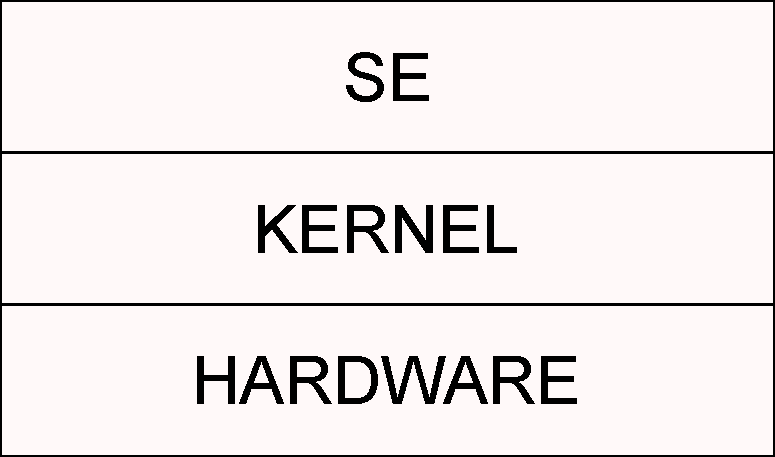
\includegraphics[width=0.75\textwidth]{images/Couches.pdf}
\end{center}

\end{frame}

\begin{frame}{\sectitle}
\begin{block}{\subsectitle}
\begin{itemize}
\item Le noyau ou kernel constitue une interface entre le matériel est les programmes
\item Il est lui même divisés en couches 
\item Il est irremplaçable par l'utilisateur
\item Il gère les processus, les périphériques, la mémoire
\end{itemize}
\end{block}

\begin{center}
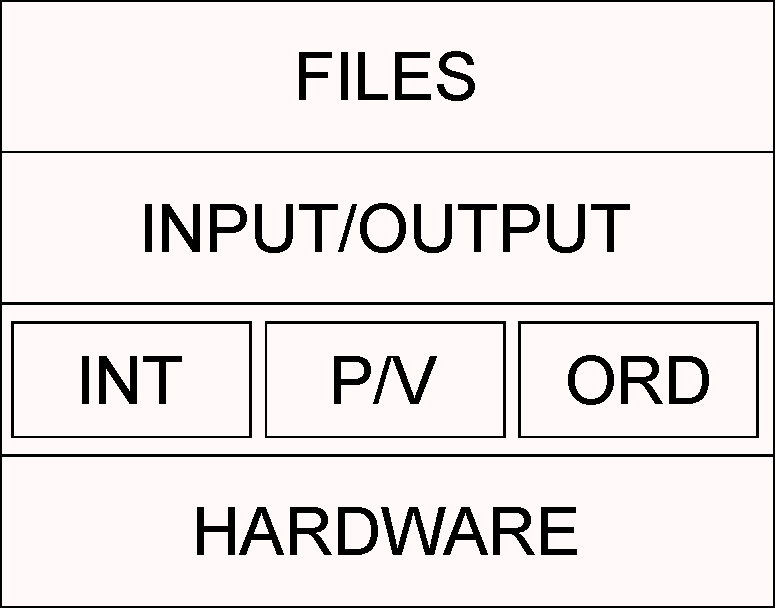
\includegraphics[width=0.50\textwidth]{images/NoyauCouches.pdf}
\end{center}

\end{frame}

%\def\sectitle{Les fichiers}
%\section{\sectitle}
\def\subsectitle{Descripteur de fichier}
\subsection{\subsectitle}
\begin{frame}{\sectitle}
	\begin{block}{\subsectitle}

		\begin{itemize}
		\item Certaines caractéristiques (la date de  création, de la dernière
modification, le  propriétaire, la  taille) sont associés aux fichiers.
		\item Stockés dans un descripteur de fichier ou index-node ou i-node.
		\item Numéro 
		\end{itemize}
	\end{block}

	\begin{alertblock}{Gestion d'inodes}
	Le système garde à un ou des emplacements connus, une table de ses inodes.
	\end{alertblock}

\end{frame}

\def\subsectitle{Les répertoires}
\subsection{\subsectitle}
\begin{frame}{\sectitle}
	\begin{block}{\subsectitle}
	Les répertoires sont une liste de (inode; nom)
	\end{block}

	\def\subsectitle{Les liens}
	\subsection{\subsectitle}
	\begin{block}{\subsectitle}
	Il existe deux types de liens :
		\begin{itemize}
		\item Hard link : c'est un pointeur sur un inode. ($\leftarrow$ on ne peut pas changer de disque)
		\item Soft link : (lien symbolique) c'est un pointeur sur le nom d'un autre fichier.
		\end{itemize}
	\end{block}

	\begin{block}{La différence}
		\begin{itemize}
		\item Les liens hards permettent d'utiliser le même contenu de fichier et d'en supprimer un sans détruire l'autre.
		\item Si le fichier source d'un lien symbolique est détruit, le lien deviens invalide.
		\end{itemize}	
	\end{block}
\end{frame}

%\def\sectitle{Droits}
%\section{\sectitle}
\def\subsectitle{Gestion des droits}
\subsection{\subsectitle}
\begin{frame}{\sectitle}
	\begin{block}{\subsectitle}
	On utilise 12 bits pour enregistrer les droits d'accès :
		\begin{itemize}
		\item [2.1.0] others
		\item [5.4.3] group
		\item [8.7.6] user
		\item [9] Sticky : laisse le programme en mémoire pour un rappel plus rapide
		\item [10] GUID : donner les mêmes droits qu'au groupe
		\item [11] SUID : donner les mêmes droits qu'à l'utilisateur
		\end{itemize}
	\end{block}
\end{frame}

\def\subsectitle{EUID et EGUID}
\subsection{\subsectitle}
\begin{frame}{\sectitle}
	\begin{block}{\subsectitle}
	Lorsque le bit SUID est activé le programme s'exécute avec l'UID du propriétaire du programme.
		\begin{itemize}
		\item Si l'UID du propriétaire est 0 : les programmes obtiens des droits root! (ex: passwd)
		\item Si le programmeur n'est pas vigilant, cela peut-être une faille de sécurité (ex: si j'arrive à lancer un terminal avec un programme SUID root: j'aurai une console superutilisateur!!)
		\end{itemize}
	\end{block}
\end{frame}

\def\sectitle{Processus}
\section{\sectitle}
\def\subsectitle{Qu'est-ce qu'un processus}
\subsection{\subsectitle}
\begin{frame}{\sectitle}
	\begin{alertblock}{\subsectitle}
	Activité associée a l'exécution d'un programme.
	\end{alertblock}
	
	\begin{block}{Ses caractéristiques}
		\begin{itemize}
		\item Contexte (temps utilisé, zone u, piles, ...)
		\item État
		\item Espace de travail
		\end{itemize}
	\end{block}
\end{frame}

\def\subsectitle{Processus et processeur}
\subsection{\subsectitle}
\begin{frame}{\sectitle}
\begin{columns}[c]
\column{.7\textwidth}
\begin{block}{\subsectitle}
Un seul processus peut avoir accès au processeur. Cela oblige certains à attendre le tour.
Un processus peut-être:
\begin{itemize}
\item Élu (c'est lui qui utilise l'UC)
\item Bloqué (il attent une entrée ou une sortie)
\item Eligible (il n'est pas bloqué, mais n'as pas le processeur)
\end{itemize}
\end{block}

\column{.3\textwidth}
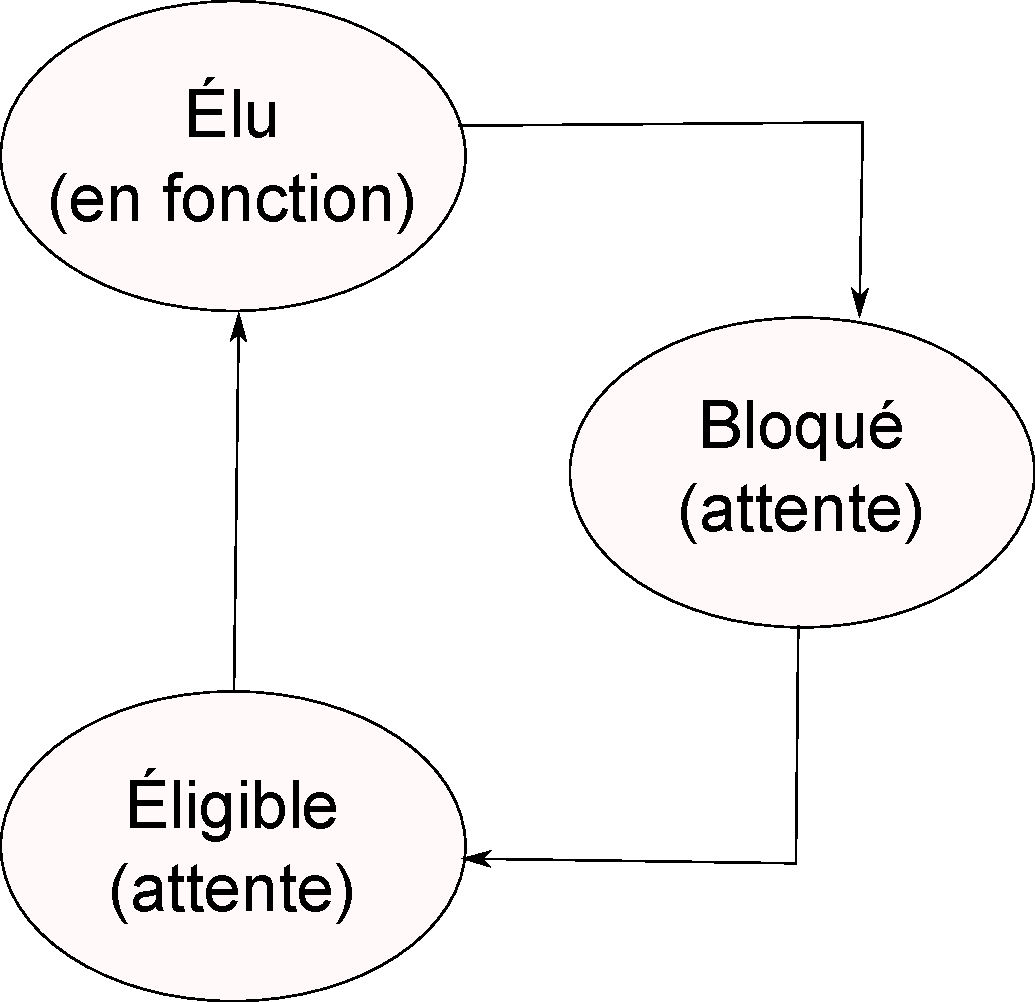
\includegraphics[width=\textwidth]{images/Status.pdf}
\end{columns}

\end{frame}



\def\subsectitle{L'espace de travail}
\subsection{\subsectitle}
\begin{frame}{\sectitle}
\begin{columns}[c]
\column{0.7\textwidth}
\begin{block}{\subsectitle}
L'espace de travail est l'ensemble des données en mémoire nécessaires à l'exécution du processus.
\begin{itemize}
\item Le code : en langage ASM, liste des instruction pour le processeurs (Pointeur: Compteur Ordinal)
\item Les données (le tas / heap) Ensemble des variables (globales/statiques/dynamiques) remplissage vers le haut
\item La pile (stack) variables des appels de fonctions (inputs, valeur avant appel (co)...) remplissage vers le bas.
\end{itemize}
\end{block}
\column{0.3\textwidth}

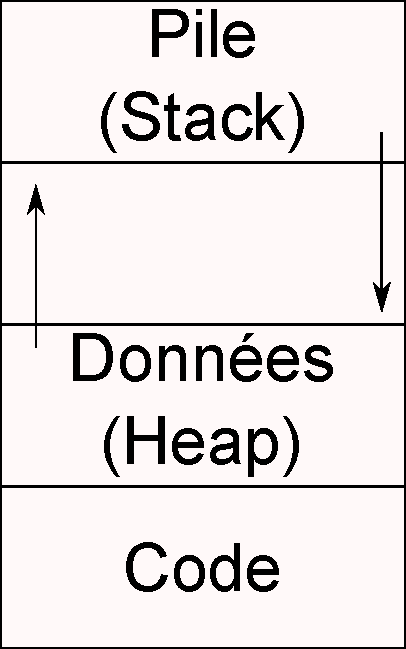
\includegraphics[width=\textwidth]{images/Workspace.pdf}
\end{columns}
\end{frame}

\def\subsectitle{La zone u}
\subsection{\subsectitle}
\begin{frame}{\sectitle}
\begin{block}{\subsectitle}
Données privées du processus. Seule la zone u du processus en cours est manipulable. (struct user <sys/user.h>)

Son adresse se trouve dans le mot état.
\begin{itemize}
\item pointeur sur la structure de processus de la table des processus. 
\item uid réel et effectif
\item Compteurs des temps (users et system) consommés
\item Masque de signaux
\item Terminal de contrôle du processus si celui-ci existe. 
\item Dernière erreur rencontrée pendant un appel système. 
\item Valeur de retour du dernier appel système. 

\end{itemize}
\end{block}
\end{frame}


\begin{frame}{\sectitle}
\begin{block}{\subsectitle}
\begin{itemize}
\item E/S (les structures associées aux entrées-sorties)
\item "." et "/" (le répertoire courant et la racine courante (c.f. chroot()) 
\item La table des descripteurs
\item imites de la taille des fichiers de la mémoire utilisable
\item umask (masque de création de fichiers)
\end{itemize}
\end{block}
\end{frame}


\def\subsectitle{Contexte}
\subsection{\subsectitle}
\begin{frame}{\sectitle}
\begin{block}{\subsectitle}
\begin{itemize}
\item son état
\item son mot d'état: en particulier
          (La valeur des registres actifs; Le compteur ordinal )
\item les valeurs des variables globales statiques ou dynamiques
\item son entrée dans la table des processus
\item sa zone u
\item Les piles user et system
\item les zones de code et de données. 
\end{itemize}
\end{block}

\begin{block}{\subsectitle}
Lorsqu'un nouveau processus va être exécuté, il y a commutation du mot d'état et changement de contexte.
Ces changements sont dictés par l'ordonnanceur.
\end{block}
\end{frame}

\begin{frame}{\sectitle}
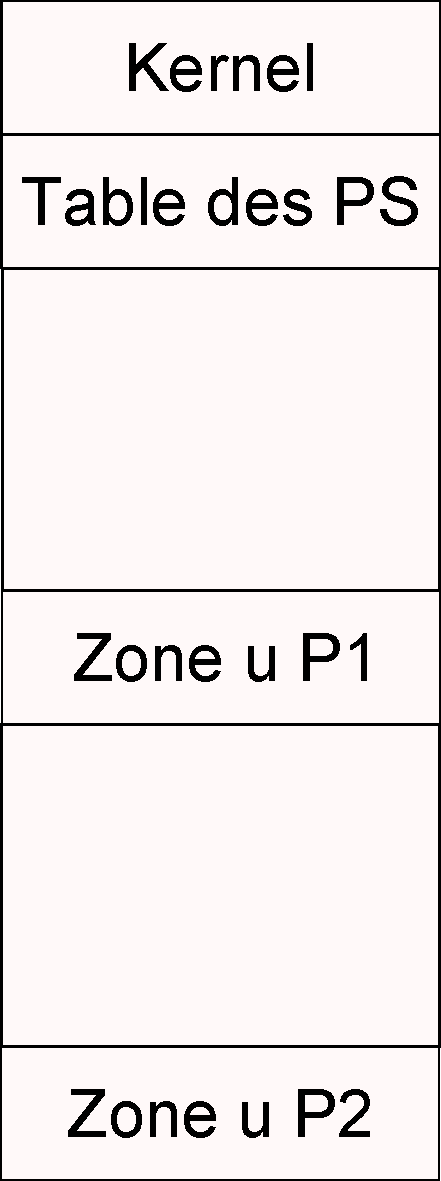
\includegraphics[height=.9\textheight]{images/TablePS.pdf}
\end{frame}

\def\subsectitle{Autres propriétés d'un processus}
\subsection{\subsectitle}
\begin{frame}{\sectitle}
\begin{block}{\subsectitle}
\begin{itemize}
\item PID
\item Descripteurs de fichiers ouverts
\item Priorité
\end{itemize}
\end{block}

\begin{block}{Decripteurs de fichiers ouverts}
\begin{itemize}
\item \verb!0 <-- /dev/term/c4! (stdin)
\item \verb!1 <-- /dev/term/c4! (stdout)
\item \verb!2 <-- /dev/term/c4! (stderr)
\item \verb!3 <-- /tmp/toto!
\end{itemize}
\end{block}
\end{frame}


\def\subsectitle{La différence entre programme et processus}
\subsection{\subsectitle}
\begin{frame}{\sectitle}
\begin{block}{\subsectitle}
Le processus est une activité d'un certain type qui possède un programme, des données en I/O et un état.
\end{block}
\end{frame}

\def\subsectitle{Hierarchie des processus}
\subsection{\subsectitle}
\begin{frame}{\sectitle}

\begin{columns}[c]
\column{.7\textwidth}
\begin{block}{\subsectitle}
Tout processus qui en créer un autre devient un père. Le processus créer est son fils.

Le processus fils hérite de tout l'environement du père (variables,  ...) sauf le PID et le PPID.
\end{block}
\column{.3\textwidth}
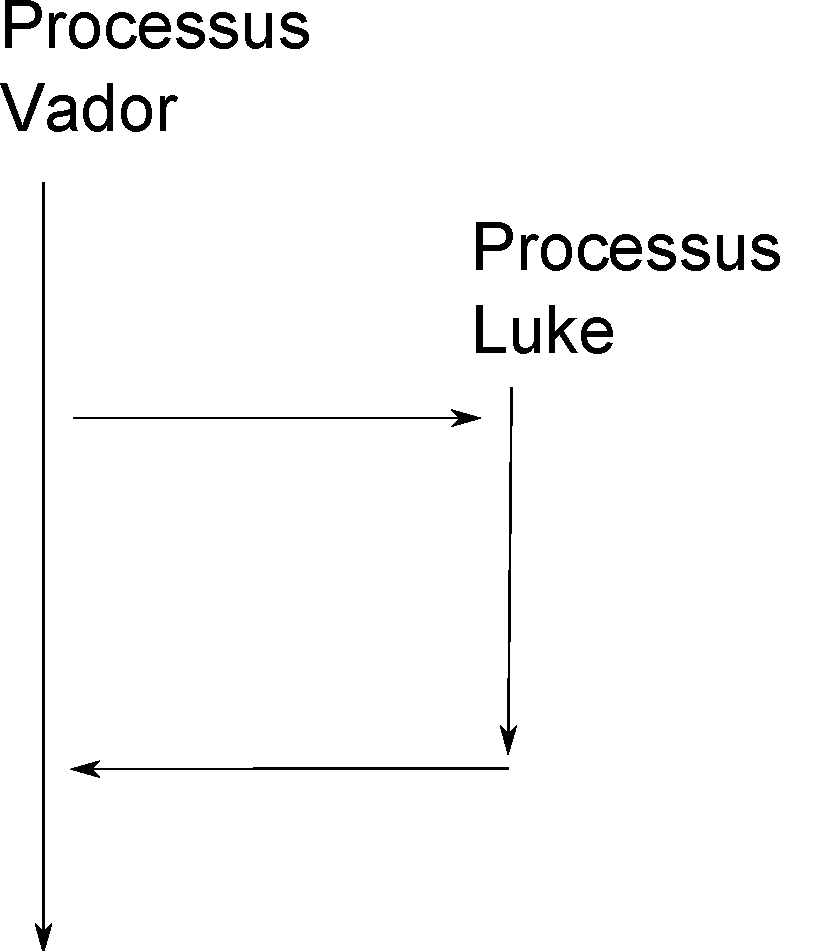
\includegraphics[width=\textwidth]{images/PereFils.pdf}
\end{columns}
\end{frame}

\begin{frame}{\sectitle}
\begin{block}{\subsectitle}
Les démons (ou daemon) sont des processus qui ne sont pas attachés à un terminal de contrôle. Ils sont souvent endormis.
On peut voir tous les processus avec la commande : \verb!ps -aux!
\end{block}

\begin{block}{\subsectitle}
Les processus père et fils peuvent fonctionner en paralèlles, ou de façon asynchrone (le père attends que le fils se termine).
En parallèle, il faut gérer les problèmes de synchronisation.
\end{block}
\end{frame}

\end{document}
